\documentclass[a4paper]{article}

\usepackage[utf8]{inputenc}
\usepackage[T1]{fontenc}
\usepackage{textcomp}
\usepackage{amsmath, amssymb}
\usepackage{tikz}

\usepackage[a4paper,
            bindingoffset=0.2in,
            left=1in,
            right=1in,
            top=1in,
            bottom=1in,
            footskip=.25in]{geometry}

\usepackage{hyperref}
\hypersetup{
    colorlinks=true,
    linkcolor=blue,
    filecolor=magenta,      
    urlcolor=cyan,
}
\title{\vspace{-2.0cm}Telecom RIO201 | Final Report}
\date{2022}
\author{Cheng-Yen Wu}

\begin{document}
\maketitle

\section{Introduction}

\subsection{Motivation}

I suffered from irregular life because I couldn't help watching drama or playing
video games until 4 AM so I'm  wondering if it exists an system of IoT
devices that can make my life more regular. At the same time, it is hard for
someone to wake up. They wake up later and then they sleep later. For me, it a
terrible cycle. My application is motivated by this scenario and I want to
provide a IoT system that can help people to rest. The functions that I wish to
enable are the followings

\begin{enumerate}
    \item It sends a pop up message on the screen when it is late. If users
        continue watching drama, it can cut the power off.
    \item It collects the sleeping information of users so that it can determine
        the quality of sleep and decide when to wake users up so that when users
        wake up, they feel less tired.
    \item It wakes users up in a peaceful way (For example, open the curtain and
        let the sunlight go into the room) and it gives a reward to users if
        they success the respact the rythme in order to show that it is not
        painful to wake up and to make it easier as a habit to sleep in time and
        wake up with power. 
\end{enumerate}

\subsection{Model and Architecture}
I model the IoT application system with three working nodes. Their functions are
described below, and the architecture is also presented in Figure
\ref{fig:architecture}.

\begin{itemize}
    \item SmartWatch: It is used to collects the sleeping data but here it
        measures the presure to simplify the model.
    \item SmartController: It connects to SmartWatch to collect the quality of
        sleep of users. Based on the data, it decides whether or not to extent
        sleep time for user. When it's the wake-up time, it turns on the light
        and open the curtain. On the other hand, at a end of day it sends a
        message to users' personal computer or TV to turn them down.
    \item SmartAppliance (light, curtain, PC or TV): It responses requests from
        SmartController and turns itself on/off.
\end{itemize}




\tikzset{every picture/.style={line width=0.75pt}} %set default line width to 0.75pt        

\begin{figure}[h] 
\centering    

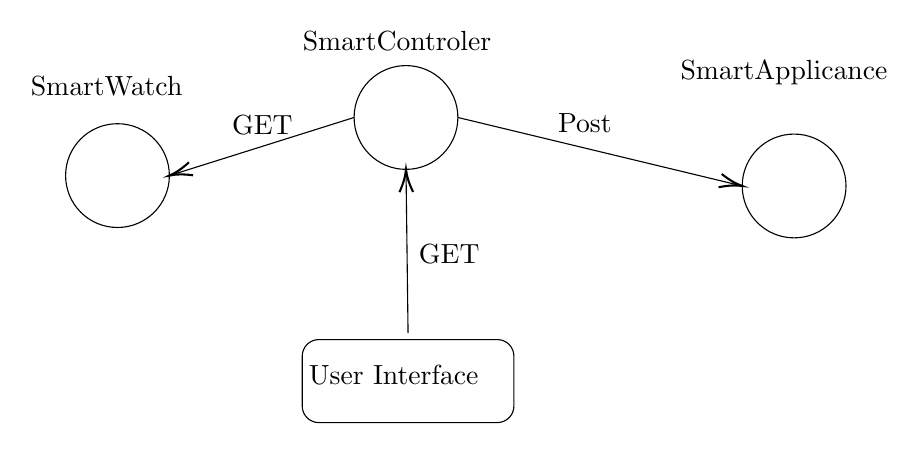
\begin{tikzpicture}[x=0.75pt,y=0.75pt,yscale=-1,xscale=1]
%uncomment if require: \path (0,277); %set diagram left start at 0, and has height of 277

%Shape: Circle [id:dp8158854378825643] 
\draw   (185,129) .. controls (185,115.19) and (196.19,104) .. (210,104) .. controls (223.81,104) and (235,115.19) .. (235,129) .. controls (235,142.81) and (223.81,154) .. (210,154) .. controls (196.19,154) and (185,142.81) .. (185,129) -- cycle ;
%Shape: Circle [id:dp47148772367248626] 
\draw   (324,101) .. controls (324,87.19) and (335.19,76) .. (349,76) .. controls (362.81,76) and (374,87.19) .. (374,101) .. controls (374,114.81) and (362.81,126) .. (349,126) .. controls (335.19,126) and (324,114.81) .. (324,101) -- cycle ;
%Shape: Circle [id:dp8925690263089208] 
\draw   (511,134) .. controls (511,120.19) and (522.19,109) .. (536,109) .. controls (549.81,109) and (561,120.19) .. (561,134) .. controls (561,147.81) and (549.81,159) .. (536,159) .. controls (522.19,159) and (511,147.81) .. (511,134) -- cycle ;
%Straight Lines [id:da9305687580429757] 
\draw    (324,101) -- (236.91,128.4) ;
\draw [shift={(235,129)}, rotate = 342.54] [color={rgb, 255:red, 0; green, 0; blue, 0 }  ][line width=0.75]    (10.93,-3.29) .. controls (6.95,-1.4) and (3.31,-0.3) .. (0,0) .. controls (3.31,0.3) and (6.95,1.4) .. (10.93,3.29)   ;
%Straight Lines [id:da37594913306206157] 
\draw    (374,101) -- (509.06,133.53) ;
\draw [shift={(511,134)}, rotate = 193.54] [color={rgb, 255:red, 0; green, 0; blue, 0 }  ][line width=0.75]    (10.93,-3.29) .. controls (6.95,-1.4) and (3.31,-0.3) .. (0,0) .. controls (3.31,0.3) and (6.95,1.4) .. (10.93,3.29)   ;
%Straight Lines [id:da21661426637906933] 
\draw    (350,204.85) -- (349.03,128) ;
\draw [shift={(349,126)}, rotate = 89.27] [color={rgb, 255:red, 0; green, 0; blue, 0 }  ][line width=0.75]    (10.93,-3.29) .. controls (6.95,-1.4) and (3.31,-0.3) .. (0,0) .. controls (3.31,0.3) and (6.95,1.4) .. (10.93,3.29)   ;
%Rounded Rect [id:dp39947486297958346] 
\draw   (299,216) .. controls (299,211.58) and (302.58,208) .. (307,208) -- (393,208) .. controls (397.42,208) and (401,211.58) .. (401,216) -- (401,240) .. controls (401,244.42) and (397.42,248) .. (393,248) -- (307,248) .. controls (302.58,248) and (299,244.42) .. (299,240) -- cycle ;

% Text Node
\draw (298,58) node [anchor=north west][inner sep=0.75pt]   [align=left] {SmartControler};
% Text Node
\draw (167,80) node [anchor=north west][inner sep=0.75pt]   [align=left] {SmartWatch};
% Text Node
\draw (480,72) node [anchor=north west][inner sep=0.75pt]   [align=left] {SmartApplicance};
% Text Node
\draw (264,99) node [anchor=north west][inner sep=0.75pt]   [align=left] {GET};
% Text Node
\draw (421,98) node [anchor=north west][inner sep=0.75pt]   [align=left] {Post};
% Text Node
\draw (354,161) node [anchor=north west][inner sep=0.75pt]   [align=left] {GET};
% Text Node
\draw (301,219) node [anchor=north west][inner sep=0.75pt]   [align=left] {User Interface};


\end{tikzpicture}
\caption{Architecture of Model}
\label{fig:architecture}

\end{figure}

\section{Implementation and demonstration}

\subsection{Implementation}
I only implemented two devices out of three in my system, SmartWatch and
SmartController. 

\begin{itemize}
    \item SmartWatch: I modelize the SmartWath with a
        \texttt{er-example-server} which sends back a sample of quality of
        sleeping at a given time. To simplify the model, it randomly gives a
        number from 0 to 9. The resource is named \texttt{new\_pressure},
        available with url \texttt{IPv6\_ADDR:5683/my\_res/new\_pressure} and is
        implemented in file \texttt{resources/res-new-pressure.c}
    \item SmartControler: I defined three phases to implement 
        SmartControler, \texttt{SLEEP} phrase, \texttt{WAKE} phrase and
        \texttt{DAY} phrase. In \texttt{SLEEP} phrase, it requests the quality
        of sleep once in a second during \texttt{SLEEP\_MAX = 8} seconds. After
        \texttt{SLEEP} phrase, the SmartController enters \texttt{WAKE} phrase.
        The first thing the SmartControler does is to determine the extension
        sleep time (XST). In my simplified model the XST is determined by sum of 8
        sample above devided by 10 seconds. After it waits XST seconds, it sends
        a message to SmartLight to turn it on and then it enters \texttt{DAY}
        phrase. It waits \texttt{24 - SLEEP\_MAX - XST} seconds. It sends message
        to PC to turn it off then it enters again \texttt{SLEEP} phrase.\\
        Users may wonder the quality of sleep. Therefore, they can connect to
        SmartControler via \texttt{CoAP GET} request. To simplify the
        implementation, the SmartControler provide the last XST. The resource is
        named \texttt{res\_new\_delay}, available with url
        \texttt{IPv6\_ADDR:5683/my\_res/new\_delay} and is implemented in file
        \texttt{resources/res-new-delay.c}. More precisely,
        \texttt{res\_new\_delay} use extern variable: \texttt{extern int
        delay\_info} to share the information between the client side and the
        server side.
\end{itemize}

The part of code related with SmartAppliance is not implemented because of lack
of time.

\subsection{Demonstration}
The demonstration is presented in the joined video \texttt{demo.webm}.  The
console above belongs to SmartWatch and the console below belongs to
SmartControler. In \texttt{demo\_delay.webm}, I showed that a user can request
the last XST via coap get API and the value is indeed equal to the latest XST.



\section{Comparison CoAP and HTTP}

I didn't have an enough time to realize an experience that can illustrate the
difference between CoAP and HTTP. Based on the slide of TP\#2, It's interesting
to count the number of packets exchanged and to measure the time of between
sending and receiving via the command \texttt{time}.

\section*{Annex}
I put my code in the folder \texttt{code}. They are
\begin{itemize}
    \item \texttt{er-example-client.c} implements SmartControler.
    \item \texttt{er-example-server.c} implements SmartWatch.
    \item \texttt{res-new-pressure.c} implements the resource
        \texttt{new\_pressure}.
    \item \texttt{res-new-pressure.c} implements the resource
        \texttt{new\_delay}.
    \item \texttt{extern\_var.h} declares the extern variable
        \texttt{delay\_info}.
\end{itemize}

    
\end{document}
